\documentclass[12pt,a4paper]{article}
\usepackage[utf8]{inputenc}
\usepackage[T1]{fontenc}
\usepackage[brazil]{babel}
\usepackage{sbc-template}
\usepackage{graphicx}
\usepackage{url}
\usepackage{hyperref}

\title{Redes veículo–oficina na gestão de frotas públicas: persistência em grafo, validação estatística de comunidades e indicadores para auditoria}
\author{Eduardo Lopes Jonker\inst{1}, Vivian Kremer Kalempa\inst{1}, Yuri Kaszubowski Lopes\inst{1}}
\address{Programa de Pós-Graduação em Computação Aplicada (PPGCAP) – Universidade do Estado de Santa Catarina (UDESC), Joinville – SC – Brasil\\ \email{eduardo.jonker@edu.udesc.br, vivian.kalempa@udesc.br, yuri.lopes@udesc.br}}

\begin{document}
\maketitle

\begin{abstract}
Public fleets serviced through accredited workshop networks generate maintenance records that can be modeled as a vehicle–workshop graph. Using real data from the Santa Catarina State Executive fleet (7.291 vehicles, 1.039 workshops), we persist the graph in Neo4j with pseudonymized identifiers, run three consistency tests and five analyses. The workshop projection has Louvain modularity Q = 0.565 versus 0.392 in degree-preserving null networks (z = 39.9), with a stable partition (mean ARI = 0.983). The top 10\% of workshops receive 69.7\% of approved spending. Workshop centrality is weakly associated with anomaly rates and the share of the budget cut in review, but communities do not differ in review cuts. The graph describes market structure and supports audit sampling; it does not, by itself, identify wrongdoing.
\end{abstract}

\begin{resumo}
Órgãos que gerenciam frotas públicas por meio de redes credenciadas de oficinas acumulam registros de manutenção que podem ser lidos como um grafo entre veículos e estabelecimentos. Este artigo constrói esse grafo com dados reais da frota do Poder Executivo de Santa Catarina (60.114 registros cobrados, 7.291 veículos e 1.039 estabelecimentos, R\$ 131,5 milhões aprovados), persiste-o em Neo4j com identificadores pseudonimizados e submete-o a três testes de consistência e a cinco análises. A projeção entre oficinas que atendem os mesmos veículos tem modularidade de Louvain Q = 0,565, contra 0,392 $\pm$ 0,004 em 30 redes nulas com a mesma sequência de graus (z = 39,9); a partição é estável entre sementes (ARI médio = 0,983). Os 10\% de oficinas com maior gasto concentram 69,7\% do valor aprovado (Gini = 0,80). A centralidade da oficina tem associação fraca e positiva com a taxa de anomalias ($\rho$ = 0,186) e com a proporção glosada do orçamento ($\rho$ = 0,172), mas não com a frequência de glosas, e as comunidades não diferem quanto a glosas (Kruskal–Wallis, p = 0,11). O grafo serve para descrever a estrutura do mercado de manutenção e para priorizar amostras de auditoria, não para identificar irregularidades por si só.

\noindent\textbf{Palavras-chave:} grafos; gestão de frotas públicas; detecção de comunidades; Neo4j; auditoria.
\end{resumo}

\section{Introdução}
A manutenção de frotas públicas no Brasil é frequentemente executada por redes de estabelecimentos credenciados, intermediadas por um sistema de gestão que registra orçamentos, aprovações e pagamentos. Em Santa Catarina, a Secretaria de Estado da Administração (SEA/SC) gerencia a frota do Poder Executivo e os contratos de gerenciamento de manutenção. Cada ordem de serviço liga um veículo a um estabelecimento, de modo que o histórico inteiro forma um grafo bipartido. Esse grafo responde a perguntas de gestão que as tabelas isoladas não respondem bem: quantas oficinas cada veículo usa, quão concentrado é o gasto, se há grupos de oficinas que atendem os mesmos veículos e se a posição de uma oficina na rede tem relação com os sinais que a fiscalização já produz.

A ciência de redes tem sido usada para estudar riscos em compras públicas, a partir de indicadores objetivos construídos com dados de contratação (Fazekas e Kocsis, 2020) e da estrutura das redes entre compradores e fornecedores (Wachs, Fazekas e Kertész, 2021). A aplicação ao pós-contrato, isto é, à execução da manutenção veicular, é menos explorada. Há também uma questão de método: algoritmos de maximização de modularidade, como o de Louvain (Blondel et al., 2008), encontram partições com modularidade alta mesmo em grafos aleatórios (Guimerà, Sales-Pardo e Amaral, 2004; Good, de Montjoye e Clauset, 2010). Sem comparação com um modelo nulo, um valor como Q = 0,56 não informa, sozinho, se há estrutura de comunidades.

Este artigo tem três objetivos: (i) materializar o grafo veículo–oficina em um banco orientado a grafos, com proteção de identificadores, e verificar que a persistência preserva a rede; (ii) testar a estrutura de comunidades contra modelos nulos e quanto à estabilidade; e (iii) medir indicadores de gestão derivados do grafo (concentração do gasto, fidelidade do veículo à oficina, centralidade) e sua associação com glosas e anomalias. O trabalho é parte de uma dissertação sobre analítica prescritiva para frotas públicas.

\section{Trabalhos relacionados}
A modularidade mede quanto as arestas internas de uma partição excedem o esperado em um grafo aleatório com os mesmos graus (Newman, 2006). O método de Louvain a maximiza de forma gulosa em duas fases (Blondel et al., 2008) e é o mais usado na prática; o método de Leiden corrige comunidades mal conectadas que o Louvain pode produzir (Traag, Waltman e van Eck, 2019). Fortunato (2010) revisa as limitações da modularidade, entre elas o limite de resolução e a degenerescência de soluções quase ótimas, que tornam importante verificar a estabilidade das partições. Para avaliar significância, a randomização por troca dupla de arestas preserva a sequência de graus (Maslov e Sneppen, 2002); a concordância entre partições é medida pelo índice de Rand ajustado (Hubert e Arabie, 1985).

Em compras públicas, Fazekas e Kocsis (2020) propõem indicadores objetivos de risco de corrupção, como propostas únicas e procedimentos não competitivos, e Wachs, Fazekas e Kertész (2021) mostram que mercados de contratação podem ser lidos como redes entre compradores e fornecedores, nas quais a estrutura de comunidades se associa ao risco. Bancos orientados a grafos representam nós, relações e propriedades explicitamente e favorecem consultas centradas em conexões (Robinson, Webber e Eifrem, 2015). Este trabalho transpõe essa leitura para a execução de contratos de manutenção, em que a unidade é o par veículo–oficina.

\section{Dados e método}
A fonte é a base processada de ordens de serviço da frota do Poder Executivo de Santa Catarina, com transações entre outubro de 2020 e julho de 2026. Foram usados os 60.114 registros com situação COBRADAS e identificadores de veículo e de estabelecimento preenchidos, de um total de 77.867 lidos. O grafo bipartido tem um nó por veículo, um por estabelecimento e uma aresta por par veículo–oficina, com o número de registros e o valor aprovado. A projeção liga duas oficinas quando atendem pelo menos dois veículos em comum, com peso igual ao número de veículos compartilhados; o limiar de dois remove coincidências isoladas.

Os identificadores de origem são substituídos por HMAC-SHA-256 com um segredo local (Krawczyk, Bellare e Canetti, 1997); placas, nomes, CPF/CNPJ, textos livres e abastecimentos não entram no grafo. O grafo é persistido em Neo4j Community 5.26, em contêiner ligado apenas ao endereço local. As análises leem as arestas do Neo4j e usam NetworkX 3.7; os indicadores por oficina (glosa e anomalia) são ligados ao grafo pela mesma pseudonimização, sem gravar identificadores originais.

A glosa é a redução entre o valor orçado e o valor aprovado de uma ordem de serviço (registro com glosa quando a diferença excede R\$ 0,05). A anomalia é a marcação de um Isolation Forest treinado na etapa de detecção de anomalias da dissertação. Os testes e as análises são:

\begin{itemize}
  \item T1 – integridade: contagens lidas do Neo4j iguais às do relatório de carga;
  \item T2 – projeção: rede entre oficinas recalculada a partir das arestas bipartidas igual à projeção gravada, aresta a aresta e peso a peso;
  \item T3 – reprodução: Louvain (semente 42) na projeção persistida comparado ao resultado do pipeline original;
  \item A1 – estabilidade: Louvain com 30 sementes, com média e desvio de Q, número de comunidades e ARI/NMI contra a semente 42;
  \item A2 – significância: Q observado contra 30 redes nulas obtidas por troca dupla de arestas (cinco trocas por aresta) com permutação dos pesos;
  \item A3 – concentração: participação das oficinas no gasto, índice de Gini, índice Herfindahl–Hirschman (HHI) e participação da oficina principal no gasto de cada veículo;
  \item A4 – auditoria: correlação de Spearman entre centralidade (grau ponderado, intermediação aproximada com 400 pivôs e número de veículos) e taxa de glosa, proporção glosada do orçamento e taxa de anomalia, para as 329 oficinas da projeção com pelo menos 30 registros, e teste de Kruskal–Wallis da taxa de glosa entre as comunidades com dez ou mais dessas oficinas;
  \item A5 – dispersão do veículo: correlação de Spearman entre o número de oficinas distintas e o custo por registro, e entre o número de oficinas e o número de registros.
\end{itemize}

\section{Resultados}
\begin{table}[ht]
\centering\small
\caption{Testes de consistência do grafo persistido}
\label{tab:t1}
\begin{tabular}{lp{0.24\linewidth}p{0.24\linewidth}p{0.24\linewidth}}
\hline
\textbf{Teste} & \textbf{Esperado} & \textbf{Observado no Neo4j} & \textbf{Resultado} \\ \hline
T1 – integridade & 7.291 veículos; 1.039 oficinas; 25.122 arestas & 7.291; 1.039; 25.122 & aprovado \\
T2 – projeção & 6.937 arestas gravadas & 6.937 recalculadas; 0 pesos divergentes & aprovado \\
T3 – reprodução & Q = 0,5646; 18 comunidades & Q = 0,5650; 19 comunidades & aprovado \\
\hline
\end{tabular}
\par\smallskip\footnotesize Fonte: Elaborado pelos autores.
\end{table}

Os três testes foram aprovados. A projeção recalculada coincide com a gravada em todas as 6.937 arestas. Densidade (0,02154) e coeficiente de agrupamento (0,0164) são iguais aos do pipeline. O Louvain produziu 19 comunidades, contra 18 no pipeline, com a mesma modularidade até a terceira casa decimal: a rede é a mesma, mas a ordem dos nós muda com as chaves pseudonimizadas, e o algoritmo é sensível a essa ordem.

O grafo bipartido mostra veículos que usam poucas oficinas e oficinas muito desiguais. A mediana é de 3 oficinas por veículo (máximo de 20); 26,9\% dos veículos usaram uma única oficina, e a oficina principal responde, na mediana, por 68,6\% do gasto do veículo. Do lado das oficinas, a mediana é de 7 veículos atendidos, o percentil 90 é de 53 e o máximo é de 806. Das 1.039 oficinas, 236 não compartilham dois veículos com nenhuma outra e ficam fora da projeção.

\begin{table}[ht]
\centering\small
\caption{Estrutura de comunidades da projeção oficina–oficina}
\label{tab:t2}
\begin{tabular}{lp{0.72\linewidth}}
\hline
\textbf{Medida} & \textbf{Valor} \\ \hline
Modularidade observada (semente 42) & 0,5650 \\
Modularidade em 30 sementes (média $\pm$ dp) & 0,5649 $\pm$ 0,0002 \\
Comunidades (mín.–máx.; moda) & 17–19; 19 \\
ARI / NMI médios contra a semente 42 & 0,983 / 0,986 \\
Modularidade em 30 redes nulas (média $\pm$ dp; máx.) & 0,3917 $\pm$ 0,0043; 0,4030 \\
Escore z do observado contra o nulo & 39,9 \\
\hline
\end{tabular}
\par\smallskip\footnotesize Fonte: Elaborado pelos autores.
\end{table}

As redes nulas, com os mesmos graus, atingem Q $\approx$ 0,39, o que confirma que modularidade alta não é, por si só, evidência de estrutura. O valor observado, porém, supera todas as 30 redes nulas por uma margem de 40 desvios-padrão: há agrupamento de oficinas por veículos compartilhados além do que os graus explicam. A partição é estável (ARI médio de 0,983), e o número de comunidades varia entre 17 e 19 conforme a semente. As cinco maiores comunidades da semente 42 têm 187, 102, 85, 83, 82 oficinas; 6 comunidades têm menos de cinco oficinas.

\begin{figure}[ht]
\centering
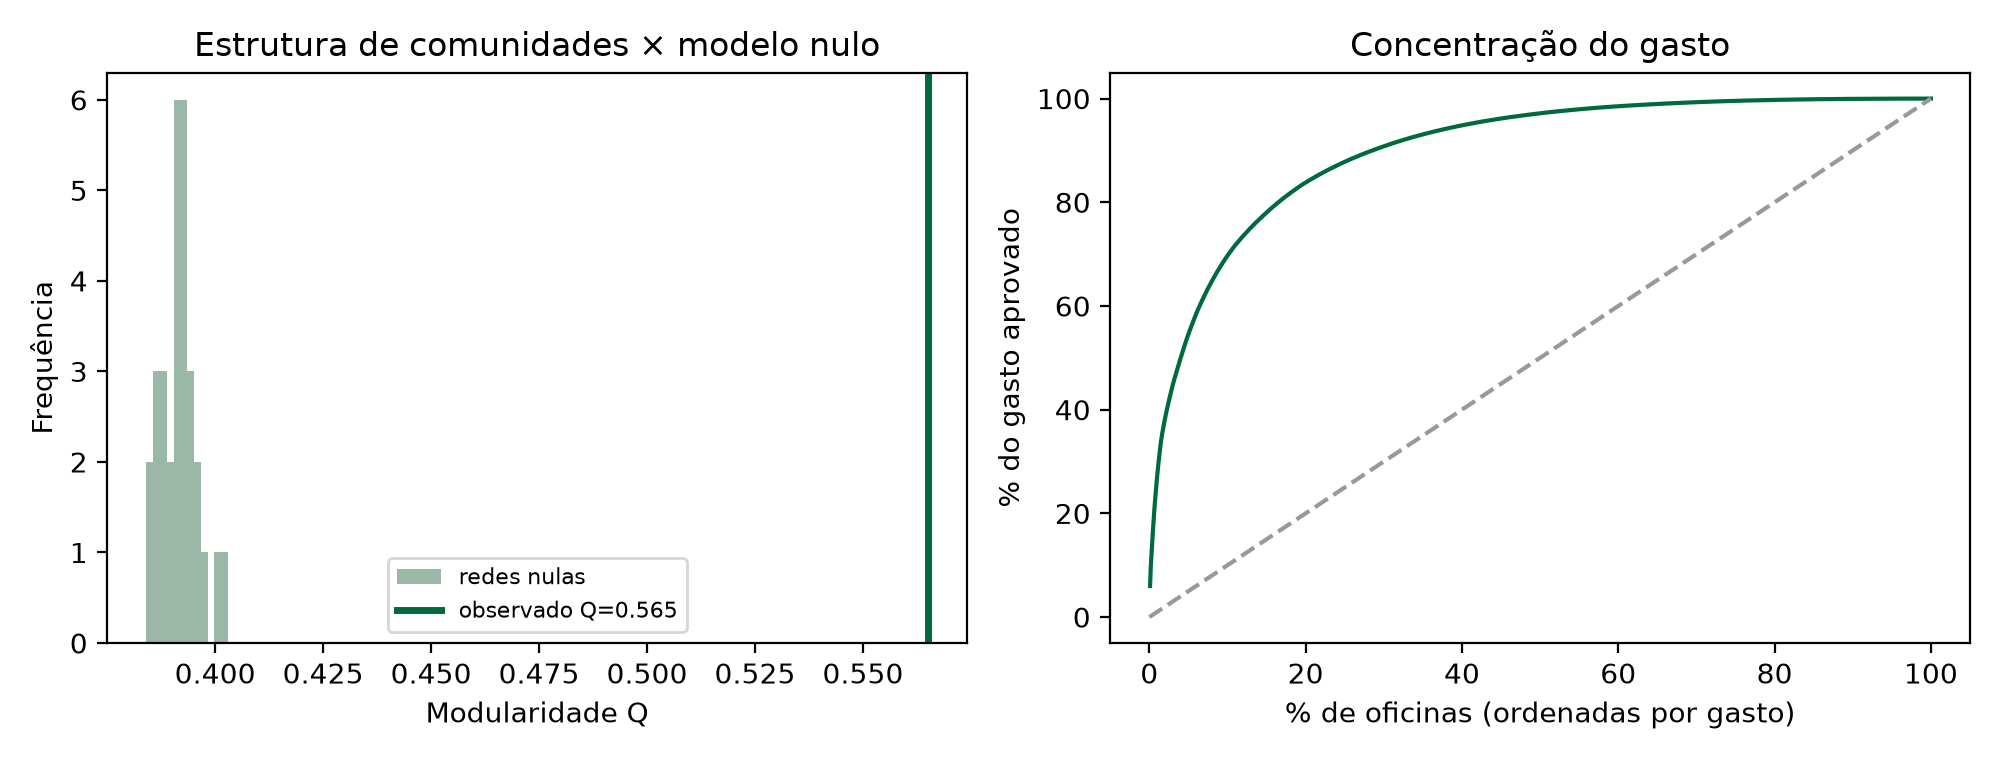
\includegraphics[width=\linewidth]{grafos_modelo_nulo_e_concentracao.png}
\caption{Modularidade observada contra as redes nulas (esquerda) e curva de concentração do gasto aprovado por oficina (direita)}
\label{fig:f1}
\par\footnotesize Fonte: Elaborado pelos autores a partir dos dados da SEA/SC.
\end{figure}

O gasto é desigual entre oficinas: os 10\% com maior gasto concentram 69,7\% do valor aprovado, as 20 maiores concentram 37,7\% e o índice de Gini é 0,80. O HHI do conjunto, de 116 pontos, é baixo porque há mais de mil estabelecimentos. Esse valor não descreve mercados locais: como o grafo não tem localização, a concentração por município ou região não pôde ser medida.

\begin{table}[ht]
\centering\small
\caption{Correlação de Spearman entre centralidade e indicadores de fiscalização (n = 329 oficinas)}
\label{tab:t3}
\begin{tabular}{lp{0.24\linewidth}p{0.24\linewidth}p{0.24\linewidth}}
\hline
\textbf{Centralidade} & \textbf{Taxa de glosa} & \textbf{Proporção glosada do orçamento} & \textbf{Taxa de anomalia} \\ \hline
Grau ponderado & 0,088 (p 0,110) & 0,138 (p 0,012) & 0,182 (p< 0,001) \\
Intermediação & 0,097 (p 0,079) & 0,172 (p 0,002) & 0,186 (p< 0,001) \\
Veículos atendidos & 0,074 (p 0,180) & 0,160 (p 0,004) & 0,146 (p 0,008) \\
\hline
\end{tabular}
\par\smallskip\footnotesize Fonte: Elaborado pelos autores. Oficinas da projeção com pelo menos 30 registros cobrados.
\end{table}

As associações são fracas. Oficinas mais centrais têm proporção um pouco maior de registros marcados como anômalos ($\rho$ entre 0,146 e 0,186) e uma fração um pouco maior do orçamento glosada ($\rho$ entre 0,138 e 0,172), mas não têm glosas mais frequentes ($\rho$ $\leq$ 0,097, p $\geq$ 0,079). A taxa de glosa também não difere entre as 8 comunidades analisadas (H = 11,66, p = 0,11).

\begin{figure}[ht]
\centering
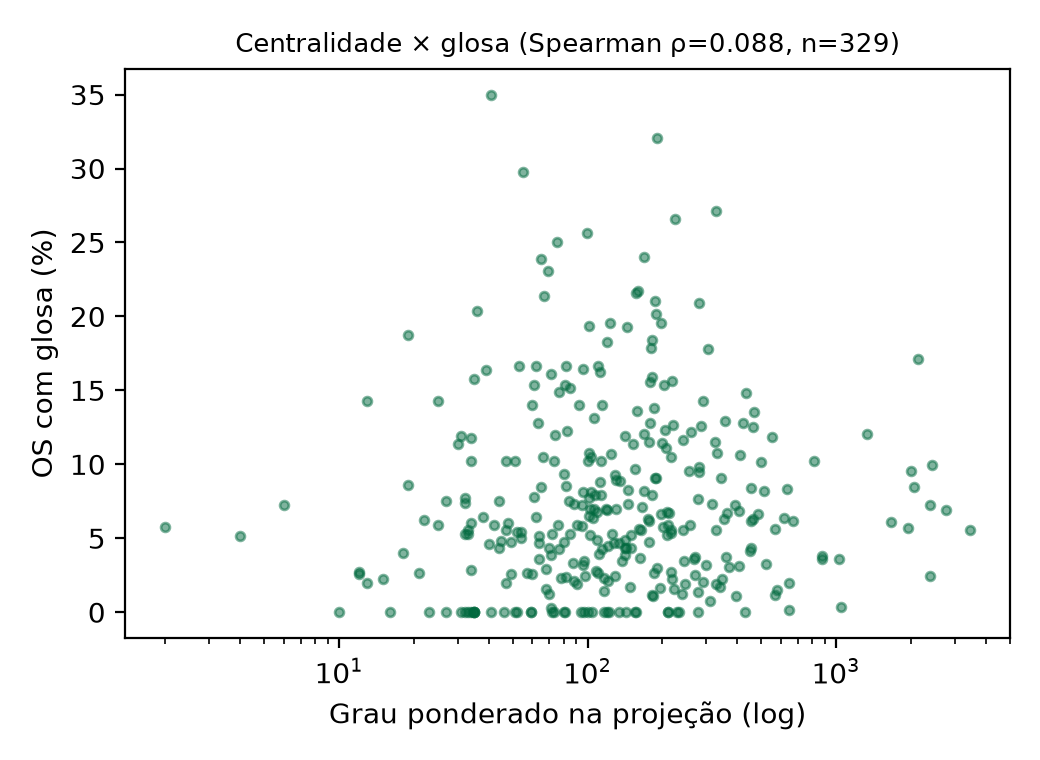
\includegraphics[width=\linewidth]{grafos_centralidade_vs_glosa.png}
\caption{Grau ponderado na projeção e percentual de ordens de serviço com glosa por oficina}
\label{fig:f2}
\par\footnotesize Fonte: Elaborado pelos autores a partir dos dados da SEA/SC.
\end{figure}

No nível do veículo, o número de oficinas cresce com o uso ($\rho$ = 0,865 com o número de registros) e tem associação fraca com o custo por registro ($\rho$ = 0,172). Veículos que passam por mais oficinas tendem a ter serviços um pouco mais caros, mas o tipo de serviço e a família do veículo, não controlados aqui, podem explicar essa diferença.

\section{Discussão}
Os resultados indicam três usos do grafo na gestão da frota. O primeiro é descritivo: a concentração do gasto e a fidelidade do veículo à oficina principal são indicadores de mercado que o gestor pode acompanhar ao longo do tempo e por órgão. O segundo é a amostragem para auditoria: comunidades estáveis e significativas delimitam grupos de oficinas que compartilham veículos e podem ser inspecionados em conjunto, e a associação fraca entre centralidade e anomalias sugere usar a centralidade como critério auxiliar de priorização, não como critério principal. O terceiro é operacional: o Neo4j torna essas relações consultáveis em Cypher pelo pessoal de controle, com identificadores protegidos.

O resultado negativo também é informativo. As comunidades não diferem quanto à frequência de glosas, e a centralidade não se associa a ela. Para o controle, isso significa que a estrutura da rede não substitui os indicadores de fiscalização e que agrupamentos densos não devem ser tratados como sinal de conluio. A leitura é compatível com a literatura de compras públicas, em que a estrutura da rede é um entre vários indicadores de risco (Fazekas e Kocsis, 2020; Wachs, Fazekas e Kertész, 2021).

O estudo tem limitações. A análise usa apenas registros cobrados, então orçamentos recusados não entram na rede. A glosa depende da fiscalização, que não é aleatória: oficinas maiores recebem mais ordens e mais revisão, e isso pode produzir parte da associação observada. A anomalia vem de um modelo não supervisionado com cerca de 1\% de marcações. A intermediação foi aproximada por amostragem de pivôs. O grafo agrega todo o período, sem dinâmica temporal, e não tem localização das oficinas. O Louvain foi usado para manter a comparação com o pipeline original; o método de Leiden (Traag, Waltman e van Eck, 2019) é a alternativa a testar.

\section{Conclusão}
O grafo veículo–oficina da frota de Santa Catarina foi persistido em Neo4j sem perda: contagens, projeção e modularidade conferem com o pipeline original. A estrutura de comunidades é real, e não um artefato do algoritmo: Q = 0,565 contra 0,392 nas redes nulas, com partição estável entre sementes. O gasto é concentrado em poucas oficinas, e cada veículo tende a depender de uma oficina principal. A centralidade se associa fracamente a anomalias e à proporção glosada, e não à frequência de glosas. Os próximos passos são incluir localização e tempo no grafo, comparar Louvain e Leiden e avaliar com a equipe da SEA/SC se as comunidades ajudam a montar amostras de auditoria.

% inicio-uso-etico-ia
\section*{Uso ético de inteligência artificial}
Os modelos de IA estudados (Isolation Forest, ensembles, SVR/SVC, SHAP, LIME, Louvain, SARIMA) usaram dados administrativos da SEA/SC com identificadores pseudonimizados (HMAC-SHA-256) e campos pessoais anonimizados, conforme a LGPD; os modelos apoiam a decisão, que cabe a um servidor responsável. No desenvolvimento, o autor usou ferramentas de IA generativa (Gemini Code Assist, GitHub Copilot, Kiro IDE e Google Antigravity IDE, no Overleaf e no Visual Studio Code) para analisar e corrigir erros de código, escrever e alterar scripts, revisar a redação e a formatação ABNT e montar slides e relatórios. Essas ferramentas não geraram dados, resultados, figuras nem hipóteses. O autor revisou todo o conteúdo gerado ou sugerido por essas ferramentas e assume integral responsabilidade pelo texto, pelo código, pelos dados e pelas conclusões deste trabalho. Declaração feita em 16/11/2026.
% fim-uso-etico-ia

\section*{Referências}
\begin{small}
BLONDEL, V. D.; GUILLAUME, J.-L.; LAMBIOTTE, R.; LEFEBVRE, E. Fast unfolding of communities in large networks. Journal of Statistical Mechanics: Theory and Experiment, v. 2008, P10008, 2008. DOI: 10.1088/1742-5468/2008/10/P10008.\par\smallskip
FAZEKAS, M.; KOCSIS, G. Uncovering high-level corruption: cross-national objective corruption risk indicators using public procurement data. British Journal of Political Science, v. 50, n. 1, p. 155-164, 2020. DOI: 10.1017/S0007123417000461.\par\smallskip
FORTUNATO, S. Community detection in graphs. Physics Reports, v. 486, p. 75-174, 2010. DOI: 10.1016/j.physrep.2009.11.002.\par\smallskip
GOOD, B. H.; DE MONTJOYE, Y.-A.; CLAUSET, A. Performance of modularity maximization in practical contexts. Physical Review E, v. 81, 046106, 2010. DOI: 10.1103/PhysRevE.81.046106.\par\smallskip
GUIMERÀ, R.; SALES-PARDO, M.; AMARAL, L. A. N. Modularity from fluctuations in random graphs and complex networks. Physical Review E, v. 70, 025101, 2004. DOI: 10.1103/PhysRevE.70.025101.\par\smallskip
HUBERT, L.; ARABIE, P. Comparing partitions. Journal of Classification, v. 2, p. 193-218, 1985. DOI: 10.1007/BF01908075.\par\smallskip
KRAWCZYK, H.; BELLARE, M.; CANETTI, R. HMAC: keyed-hashing for message authentication. RFC 2104. IETF, 1997. DOI: 10.17487/RFC2104.\par\smallskip
MASLOV, S.; SNEPPEN, K. Specificity and stability in topology of protein networks. Science, v. 296, p. 910-913, 2002. DOI: 10.1126/science.1065103.\par\smallskip
NEWMAN, M. E. J. Modularity and community structure in networks. Proceedings of the National Academy of Sciences, v. 103, p. 8577-8582, 2006. DOI: 10.1073/pnas.0601602103.\par\smallskip
ROBINSON, I.; WEBBER, J.; EIFREM, E. Graph databases: new opportunities for connected data. 2. ed. Sebastopol: O'Reilly Media, 2015.\par\smallskip
TRAAG, V. A.; WALTMAN, L.; VAN ECK, N. J. From Louvain to Leiden: guaranteeing well-connected communities. Scientific Reports, v. 9, 5233, 2019. DOI: 10.1038/s41598-019-41695-z.\par\smallskip
WACHS, J.; FAZEKAS, M.; KERTÉSZ, J. Corruption risk in contracting markets: a network science perspective. International Journal of Data Science and Analytics, v. 12, p. 45-60, 2021. DOI: 10.1007/s41060-019-00204-1.\par\smallskip
\end{small}
\end{document}
